\scanpage{40}
\mspage{\handwritten{23}}
% archive sheet number: 39 (inverted, upper left)
% The two loop-and-stem signs below reproduce the handwritten linking marks; they are not read as letters.
% The top and bottom marginal continuations are placed at their marked insertion points.
sent en termes de limites projectives finies exclusivement, tandis que les autres notions impliquent implicitement des constructions faisant appel également à des limites ind\unsure{\deleted{c}u|u}\unsure{\deleted{u}c|c}tive\unsure{\deleted{s}s|s})\handwritten{)}.
\inserted{\handwritten{De plus, le foncteur $u^{*}$ ``\uline{commute}'' à toutes
\tikz[baseline=-0.3ex,scale=.18]{\draw (0,1.3)--(0,.15) .. controls (-.4,-.2) and (.4,-.2) .. (0,.15);}
\figure{\begin{tikzpicture}
\node[inner sep=6pt,text width=.88\linewidth,align=left] (n) {\tikz[baseline=-0.3ex,scale=.18]{\draw (0,1.3)--(0,.15) .. controls (-.4,-.2) and (.4,-.2) .. (0,.15);}les opérations fonctorielles \deleted{\illegible{1}} habituelles faites en termes de telles structures, plus précisément à toutes les opérations qui \inserted{peuvent} s'exprime\deleted{nt}\unsure{r} en termes de $\varinjlim$ et de $\varprojlim$ finies: constructions d'objets libres (groupes ou modules libres, p.ex.) engendrés par un objet, produits tensoriels (cf. \S 6 plus bas) etc.};
\draw ([yshift=2mm]n.north west) .. controls ([xshift=-2mm]n.west) and ([xshift=-1mm]n.south west) .. (n.south west) -- ([xshift=1mm]n.south) -- ([xshift=2mm,yshift=2mm]n.south) -- ([yshift=2mm]n.south east);
\end{tikzpicture}}}}

\margin{\handwritten{\figure{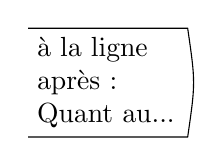
\begin{tikzpicture}\node[align=left,text width=1.8cm,inner sep=3pt] (n) {à la ligne après : Quant au...};\draw (n.north west)--(n.north east) .. controls ([xshift=1mm]n.east) .. (n.south east)--(n.south west);\end{tikzpicture}}}}
% The opposing pen brackets mark the paragraph break immediately before Quant au.
\handwritten{\tikz[baseline=-.6ex,scale=.18]{\draw (0,1.5)--(.5,1.4)--(.6,0)--(0,-.15);\draw (1.4,1.4)--(.9,1.35)--(.9,-.1)--(1.5,-.15);}}
Quant au foncteur image directe $\mathrm{u}_{\handwritten{*}}$\inserted{$:\mathrm{E}\handwritten{\longrightarrow}\mathrm{E}'$}, qui commute aux limites projectives, il ``respecte'' \inserted{par suite} toute structure algébrique sur un objet (ou une famille d'objets) de $\mathrm{E}$, définissable en termes de limites projectives \inserted{exclusivement} (telles les str\deleted{i}uctures de groupe, d'anneau ou de module sur un anneau, \deleted{dans}\inserted{parmi} les exemples précédents). Par \deleted{f}contre, le foncteur $\mathrm{u}_{\handwritten{*}}$ n\deleted{e}'est en général pas exact à droite i.e. il ne commute pas en général aux limites inductives finies, et même ne transforme pas en général épimorphisme en épimorphisme\handwritten{\unsure{;|,}} (c'est d'ailleurs \deleted{\unsure{comme} nous le verrons au} ce défaut d'exactitude du foncteur $\mathrm{u}_{\handwritten{*}}$ qui est \handwritten{à} la source de ces propriétés cohomologiques, qui seront étudiées (du point de vue de l'algèbre homologique commutative) dans l'exposé suivant\handwritten{)}.
\inserted{\handwritten{Par suite, il ne \deleted{transforme pas}\inserted{s'étend pas}, en général,
\tikz[baseline=-.3ex,scale=.18]{\draw (0,0)--(.05,1.3) .. controls (-.35,1.65) and (.45,1.65) .. (.05,1.3);}
\figure{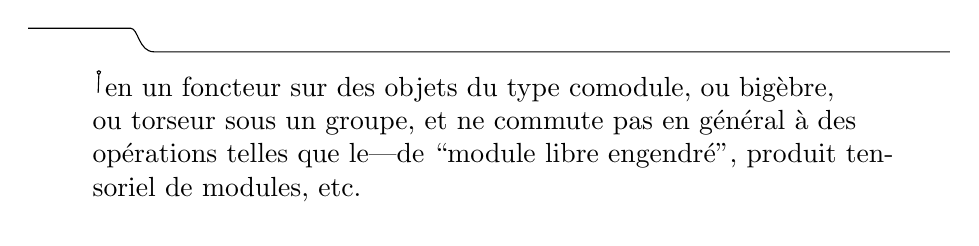
\begin{tikzpicture}
\node[inner sep=6pt,text width=.88\linewidth,align=left] (n) {\tikz[baseline=-.3ex,scale=.18]{\draw (0,0)--(.05,1.3) .. controls (-.35,1.65) and (.45,1.65) .. (.05,1.3);}en un foncteur sur des objets du type comodule, ou bigèbre, ou torseur sous un groupe, et ne commute pas en général à des opérations telles que \deleted{\unsure{le|de}} ``module libre engendré'', produit tensoriel de modules, etc.};
\draw ([xshift=-6mm,yshift=3mm]n.north west)--([xshift=7mm,yshift=3mm]n.north west) .. controls ([xshift=8mm,yshift=3mm]n.north west) and ([xshift=8mm]n.north west) .. ([xshift=10mm]n.north west)--(n.north east);
\end{tikzpicture}}}}

\deleted{2}\handwritten{3}.1.\handwritten{3}. En pratique, lorsqu'on \deleted{se donne}\inserted{est \inserted{\handwritten{en}} présenced'}un foncteur $\mathrm{f}:\mathrm{E}\handwritten{\longrightarrow}\mathrm{F}$ d'un $\underline{\mathrm{U}}$-topos dans un autre, il y a lieu d'en expliciter \inserted{\handwritten{toutes}} les propri\deleted{t}é\deleted{é}tés d'exactitude, \deleted{y compris et de déterminer s'il admet un foncteur exact} y compris l'existence éventuelle de foncteurs adjoints à gauche ou à droite (cf. la note de bas de page précédente), pour parvenir à une compréhension de la ``nature géométrique'' de $\mathrm{f}$, \deleted{qui} compréhension qui sera généralement un guide indispensable pour \deleted{l'}\inserted{une}intuition géométrique correcte de la situation. Ainsi, s'il s'avère que $\mathrm{f}$ commute aux limites inductives quelconques et aux limites projectives finies, il y a lieu d'écrire $\mathrm{f}$ sous la forme
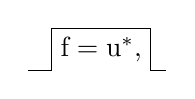
\begin{tikzpicture}[baseline=(n.base)]\node[inner sep=3pt] (n) {$\mathrm{f}=\mathrm{u}^{\handwritten{*}}$,};\handwritten{\draw ([xshift=-3mm]n.south west)--(n.south west)--(n.north west)--(n.north east)--(n.south east)--([xshift=2mm]n.south east);}\end{tikzpicture}
où
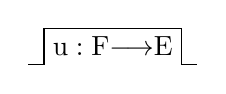
\begin{tikzpicture}[baseline=(n.base)]\node[inner sep=3pt] (n) {$\mathrm{u}:\mathrm{F}\handwritten{\longrightarrow}\mathrm{E}$};\handwritten{\draw ([xshift=-2mm]n.south west)--(n.south west)--(n.north west)--(n.north east)--(n.south east)--([xshift=2mm]n.south east);}\end{tikzpicture}
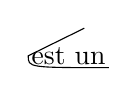
\begin{tikzpicture}[baseline=(n.base)]\node[inner sep=1pt] (n) {est un};\handwritten{\draw ([xshift=2mm,yshift=2mm]n.north)--(n.west) .. controls (n.south west) .. (n.south east);}\end{tikzpicture}
morphisme de topos, i.e. d'interpréter $\mathrm{f}$ comme un foncteur ``image inverse'' par une ````application continue'' de topos. Lorsque $\mathrm{f}$ commute aux limites projectives quelconques, donc qu'il admet un adjoint à gauche,\deleted{$\mathrm{g}$}
